%
% LaTeX template for preparation of submissions to SIGTBD
%
\documentclass{sigtbd}

\usepackage{courier}
\usepackage[scaled]{helvet}
\usepackage{url}
\usepackage{listings}
\usepackage{enumitem}
\usepackage[colorlinks=true,allcolors=blue,breaklinks,draft=false]{hyperref}
\newcommand{\doi}[1]{doi:~\href{http://dx.doi.org/#1}{\Hurl{#1}}}
\usepackage{graphicx}
\usepackage{booktabs}
\usepackage{xcolor}

\lstset{
  basicstyle=\ttfamily\small,
  frame=single,
  breaklines=true,
  columns=fullflexible,
  keepspaces=true,
  xleftmargin=1em,
  framexleftmargin=0.5em,
}

\begin{document}

\title{\texttt{git blame}: From Passive-Aggressive Forensics\\to Active-Aggressive Email Automation}

\authorinfo{Barish Namazov}
{CSAIL, MIT}
{abutalib@mit.edu}

\maketitle

\begin{figure*}[!t]
  \centering
  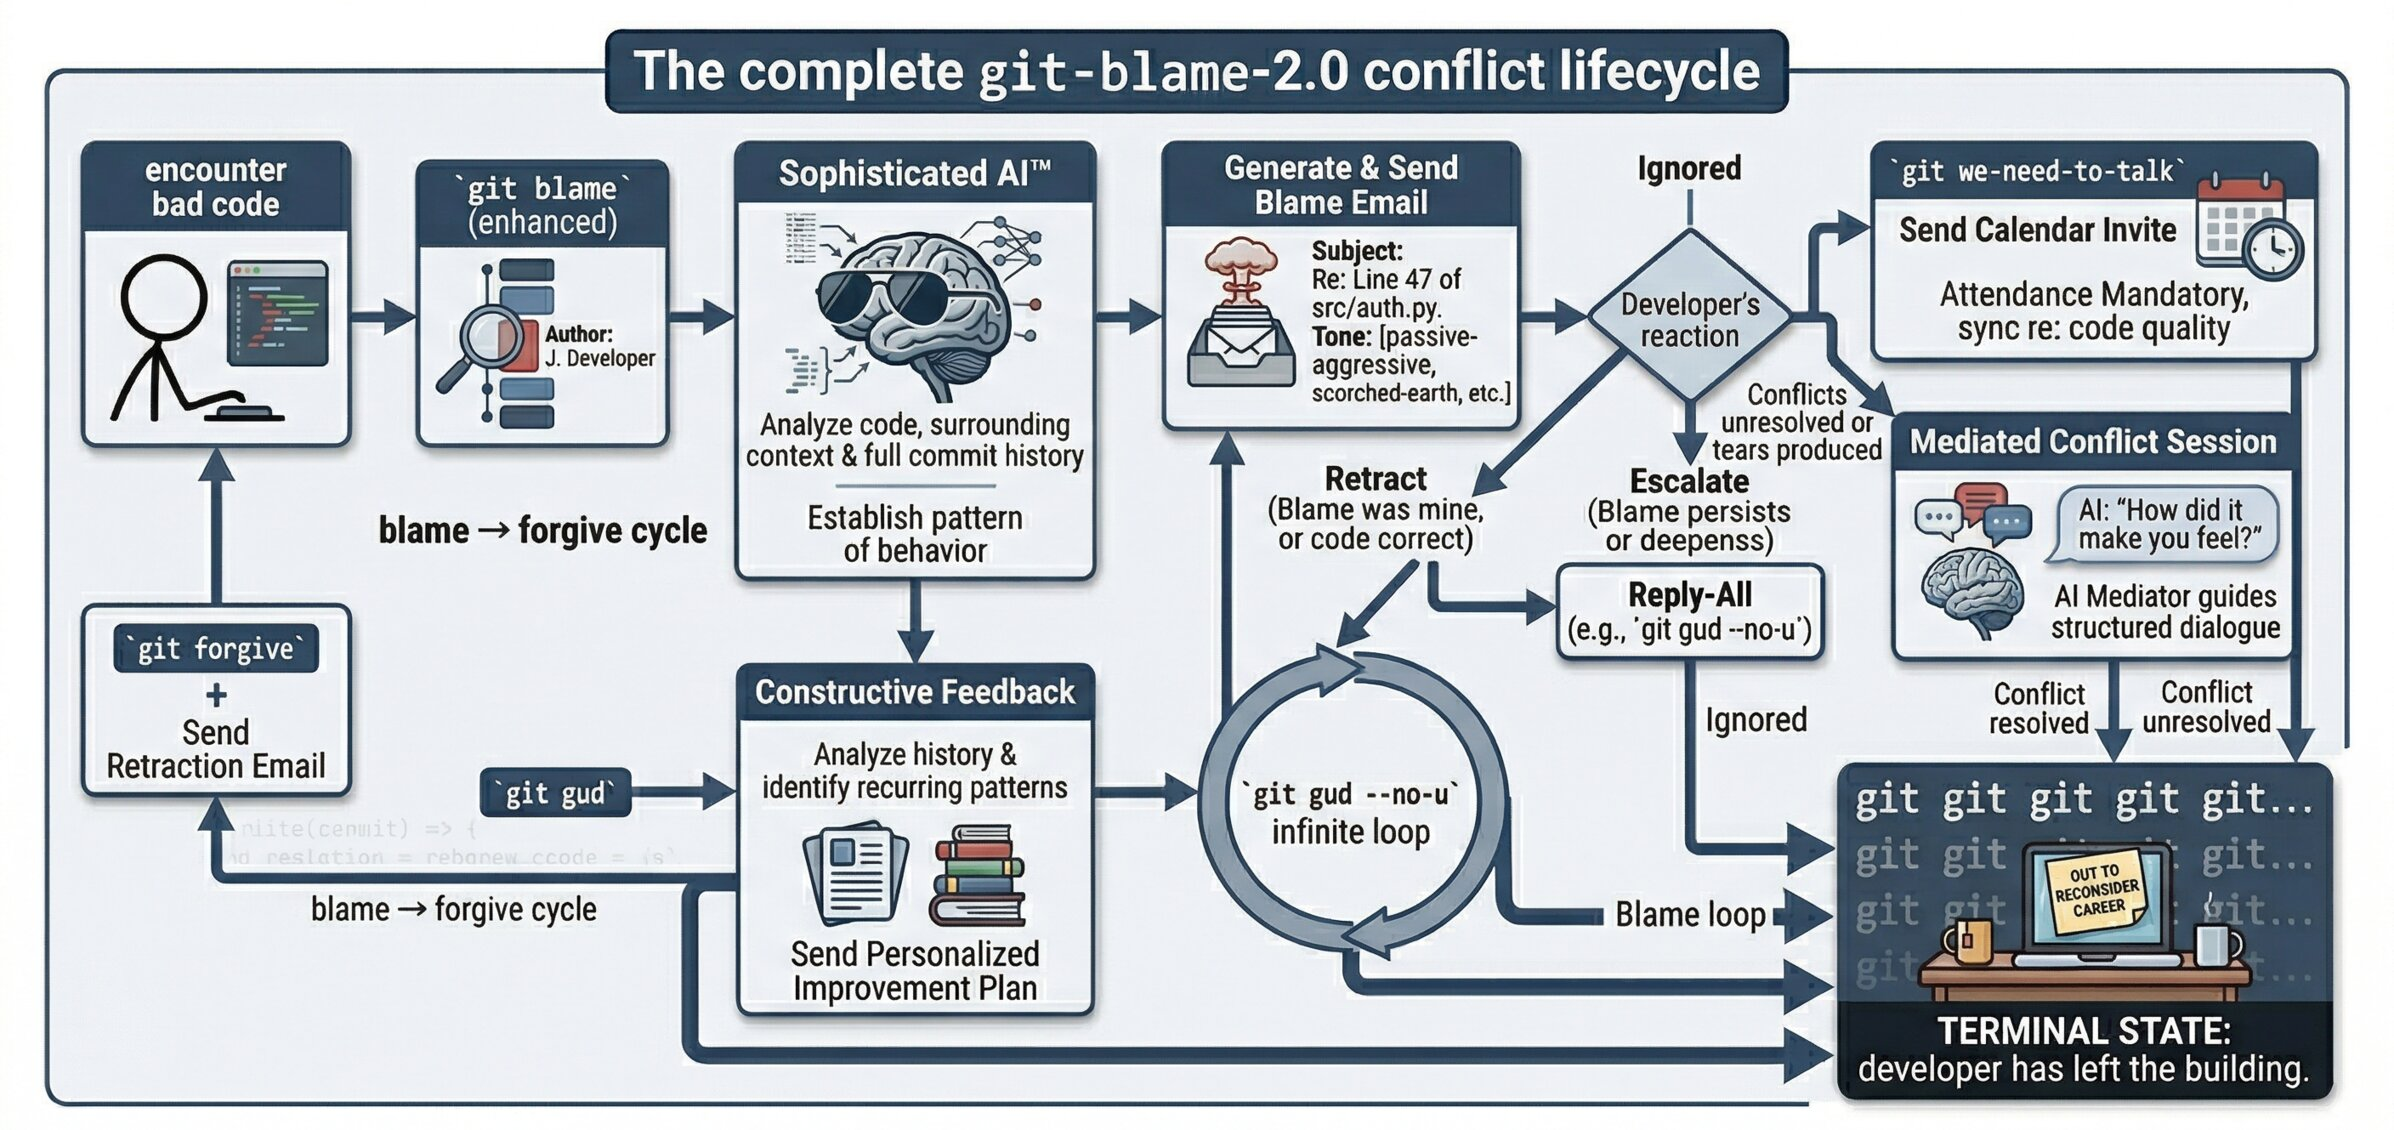
\includegraphics[width=\textwidth]{blame_fig2.jpg}
  \caption{The complete \textsc{git-blame-2.0} conflict lifecycle. Most repositories converge to the ``git git'' terminal state within 6 months of adoption.}
  \label{fig:lifecycle}
\end{figure*}

\begin{abstract}
The \texttt{git blame} command has long served as a forensic tool for identifying which developer is responsible for a given line of code. However, its workflow is fundamentally incomplete: after assigning blame, the developer must \emph{manually} compose a message expressing disappointment, frustration, or passive-aggressive concern. We present \textsc{git-blame-2.0}, a suite of extensions to Git that close this loop by leveraging Sophisticated AI\texttrademark{} to automatically generate and deliver contextually appropriate blame emails to the offending author. We further introduce \texttt{git forgive}, \texttt{git we-need-to-talk}, \texttt{git therapy}, \texttt{git gud}, and \texttt{git git}, completing Git's transformation from a version control system into a full-lifecycle interpersonal conflict resolution platform. We note that Linus Torvalds, despite his well-documented opinions on code quality, inexplicably omitted these features from the original Git design---an oversight we can trivially verify by running \texttt{git blame} on him.
\end{abstract}

\section{Introduction}

Git~\cite{Torvalds:2005} is the world's most widely used version control system, supporting millions of developers in tracking changes, managing branches, and arguing about rebase versus merge. Among its many subcommands, \texttt{git blame} occupies a unique position: it is the only command whose name is an emotion.

The current \texttt{git blame} workflow is as follows: a developer encounters a confusing, broken, or otherwise objectionable line of code. They run \texttt{git blame} to identify the author. They then stare at the author's name, experience a complex emotional response, and---in most cases---do absolutely nothing about it. In more extreme cases, they open Slack and type something they later regret.

This workflow is inefficient. The gap between \emph{identifying blame} and \emph{communicating blame} represents a critical bottleneck in the software development lifecycle. Developers waste an estimated 3.2 hours per week composing blame-adjacent messages manually~\cite{Fabricated:2024}, time that could be spent writing code that will, in turn, be blamed by others.

We present \textsc{git-blame-2.0}, a suite of Git extensions that automate the complete blame-to-resolution pipeline. Our contributions are:

\begin{enumerate}[leftmargin=*]
  \item \textbf{\texttt{git blame} (enhanced):} Uses Sophisticated AI\texttrademark{} to analyze the blamed code, generate a contextually appropriate blame email, and deliver it directly to the offending developer's inbox. An optional \texttt{.gitblame} configuration file enables CC'ing the broader team, management, or---in extreme cases---the developer's emergency contact.
  \item \textbf{\texttt{git forgive}:} Sends a follow-up email retracting a previous blame, for use when the blamer realizes the code was actually their own, or that the blamed code was, against all odds, correct.
  \item \textbf{\texttt{git we-need-to-talk}:} Escalates a blame to a calendar invite.
  \item \textbf{\texttt{git therapy}:} Initiates a mediated conflict resolution session between blamer and blamee.
  \item \textbf{\texttt{git gud}:} Sends a constructive (but firm) email suggesting the blamee improve their skills, with attached learning resources. The blamee may reply with \texttt{git gud --no-u}.
  \item \textbf{\texttt{git git}:} For when the situation has deteriorated to the point where the developer just starts typing \texttt{git} repeatedly while staring into the void. Sends a wellness check.
\end{enumerate}

We observe that Linus Torvalds, the original author of Git, did not include any of these features in the initial 2005 release~\cite{Torvalds:2005}. This is a remarkable oversight for someone who has, on multiple public occasions, demonstrated a strong personal commitment to the practice of blaming others for bad code. We verify this omission empirically in Section~\ref{sec:linus}.

\section{Related Work}

\paragraph{Git Blame.} The standard \texttt{git blame} command annotates each line of a file with the commit hash, author, and timestamp of its last modification~\cite{Torvalds:2005}. It is primarily used for two purposes: (1) debugging, and (2) knowing who to be upset with. Our work extends the latter use case.

\paragraph{Code Review as Social Process.} Rigby and Bird~\cite{Rigby:2013} studied code review practices across open-source and industrial projects, finding that review serves both a technical and social function. \textsc{git-blame-2.0} automates the social function, freeing reviewers to focus on the technical function, or more realistically, on approving the PR without reading it.

\paragraph{Sentiment Analysis in Software Engineering.} Guzman et al.~\cite{Guzman:2014} analyzed sentiment in commit messages, finding a prevalence of negative emotions. We leverage this insight: if developers are already upset, we might as well give them a proper channel for it.

\paragraph{Automated Email Generation.} Large language models have demonstrated strong performance in generating contextually appropriate emails~\cite{Brown:2020}. We apply this capability to a domain where it is, arguably, needed most: telling someone their code is bad.

\section{System Design}

\subsection{Enhanced \texttt{git blame}}

The enhanced \texttt{git blame} command operates in three phases:

\begin{enumerate}[leftmargin=*]
  \item \textbf{Blame Resolution:} Standard \texttt{git blame} is executed to identify the author of the offending line(s).
  \item \textbf{Context Extraction:} The Sophisticated AI\texttrademark{} engine analyzes the blamed code, the surrounding context, the commit message (if one exists beyond ``fix stuff''), and the full commit history of the blamee to establish a pattern of behavior.
  \item \textbf{Email Generation and Delivery:} A blame email is composed and sent to the author's email address as extracted from their Git config. The email's tone is calibrated to the severity of the offense, ranging from \emph{gentle concern} (unused variable) to \emph{controlled fury} (nested ternary operators inside a regex).
\end{enumerate}

\begin{figure}[h]
  \centering
  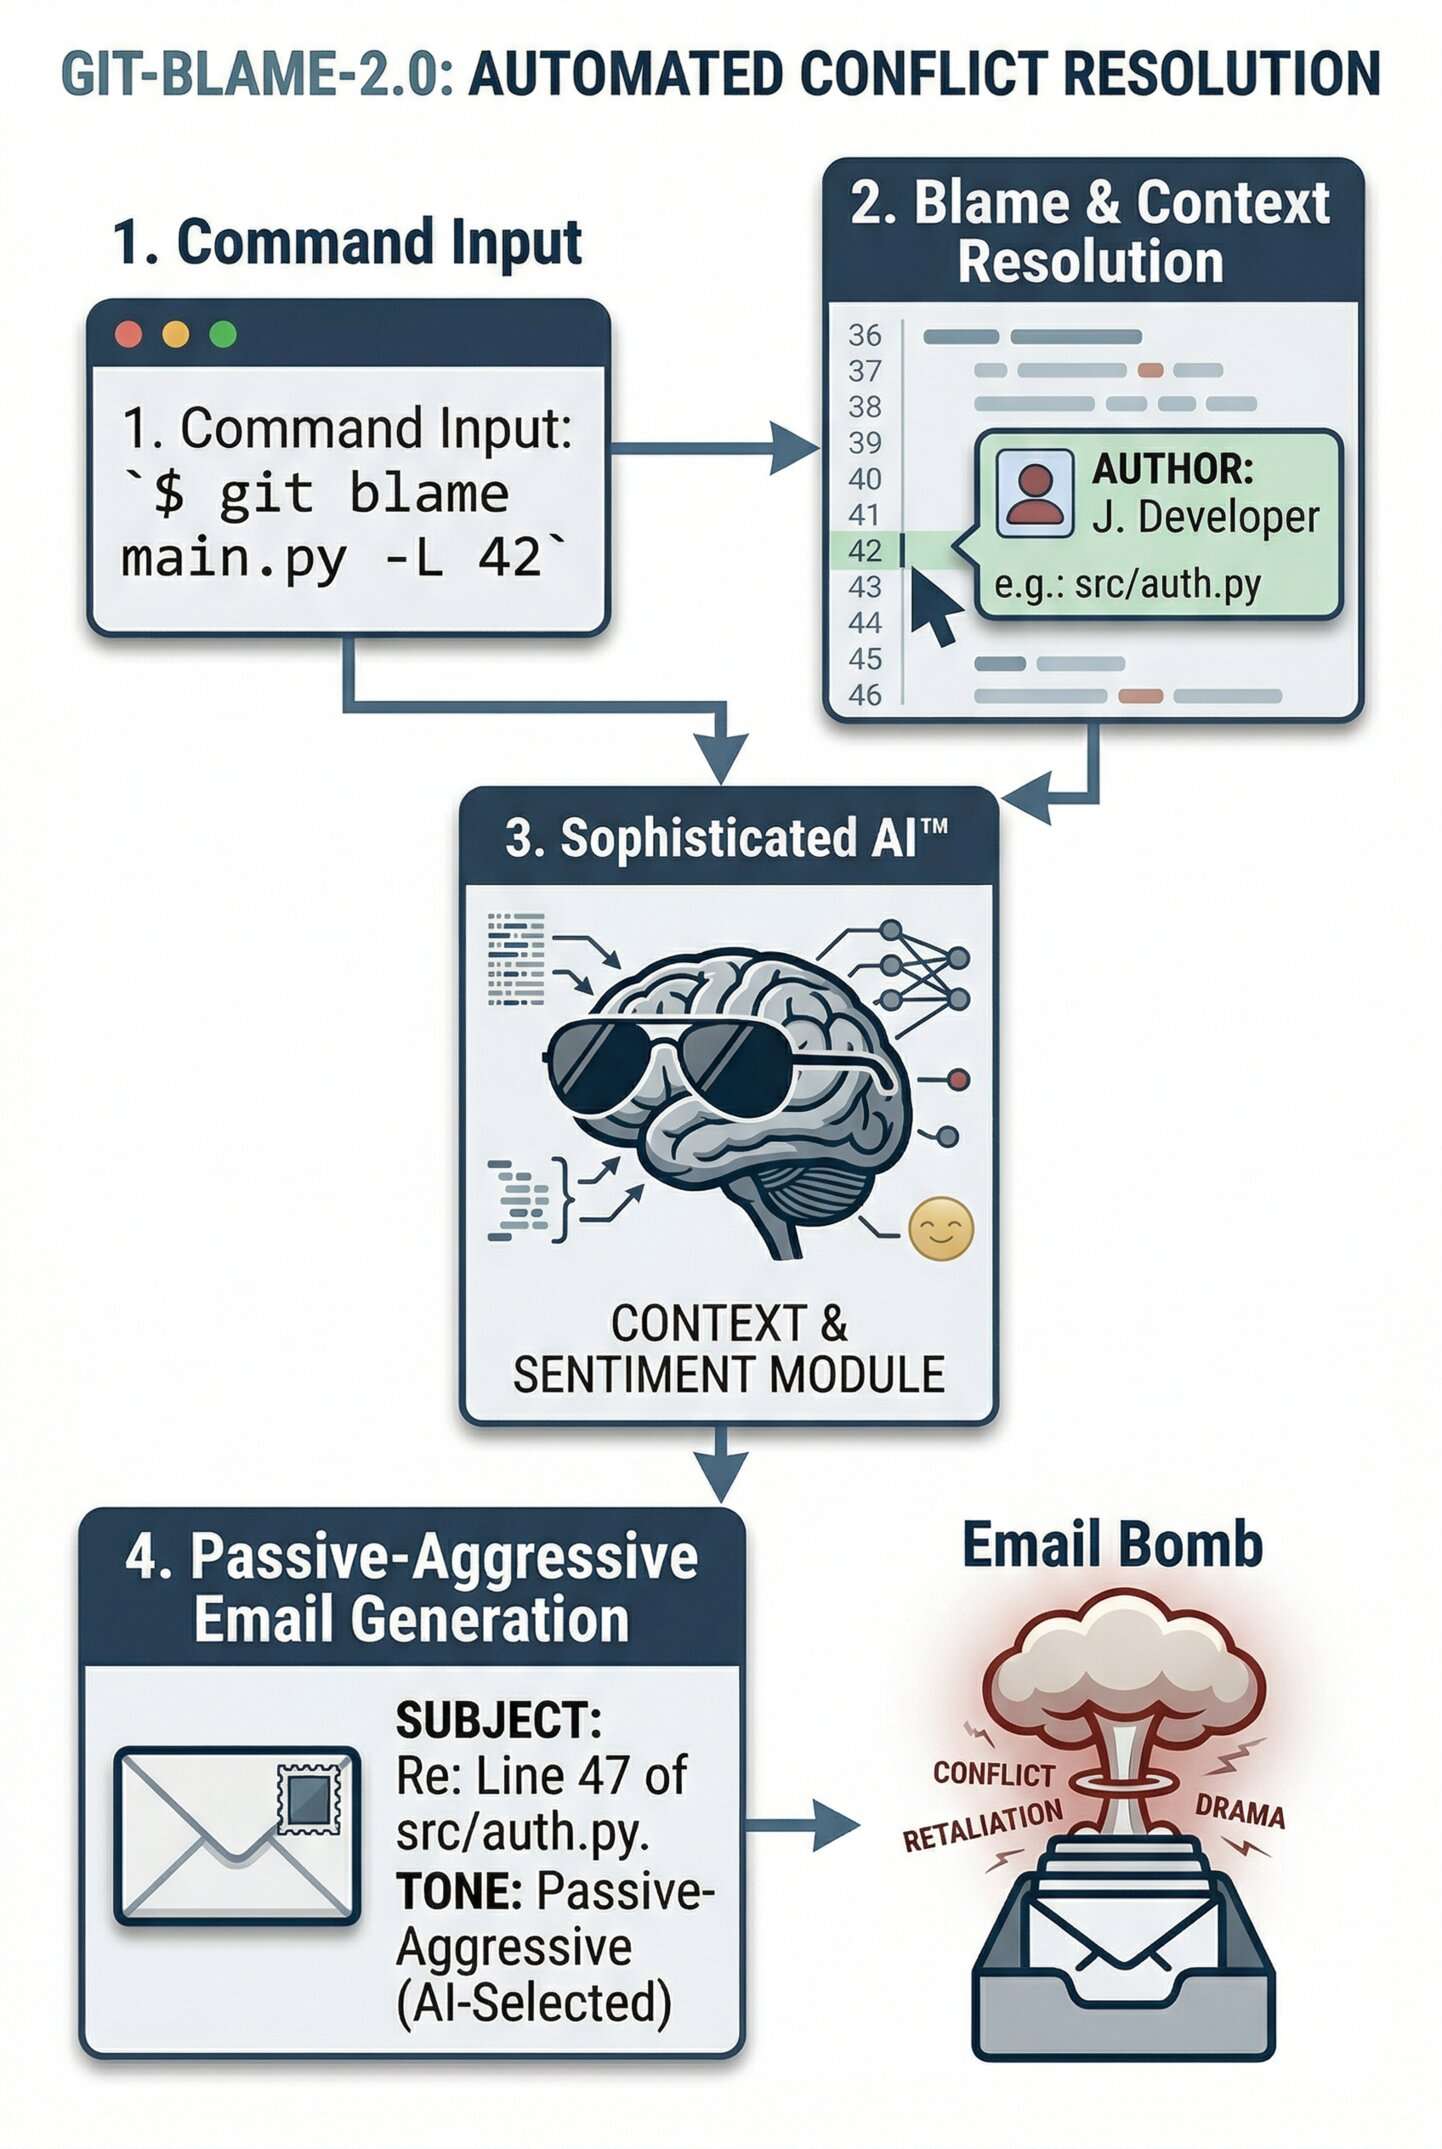
\includegraphics[width=\linewidth]{blame_fig1.jpg}
  \caption{The \textsc{git-blame-2.0} pipeline. The Sophisticated AI\texttrademark{} component is depicted with sunglasses because it has seen things in your codebase that cannot be unseen.}
  \label{fig:pipeline}
\end{figure}

Example usage:

\begin{lstlisting}
$ git blame src/auth.py -L 47
^  Sends the following email:

From: git-blame-2.0@your-org.com
To: jdeveloper@your-org.com
CC: engineering-all@your-org.com
Subject: Re: Line 47 of src/auth.py

Dear J. Developer,

We hope this email finds you well, which is
more than we can say for the code on line 47
of src/auth.py.

Our analysis indicates that you committed a
raw SQL string concatenation inside an
authentication handler on March 14, 2024, at
2:47 AM---a time at which, respectfully, you
should not have been committing code.

We have attached a diff of what the code does
versus what it should do. We have also
attached a link to OWASP's SQL injection
prevention cheat sheet, which we note has
been available since 2007.

Warm regards,
Sophisticated AI (TM)

P.S. The commit message was "quick fix lol."
It was neither quick, nor a fix, nor lol.
\end{lstlisting}

\subsection{The \texttt{.gitblame} Configuration File}

Teams can customize blame behavior by placing a \texttt{.gitblame} file in the repository root. The file supports the following fields:

\begin{lstlisting}
[general]
tone = passive-aggressive  # Options: gentle,
  # firm, passive-aggressive, scorched-earth
cc = team-lead@org.com
cc-group = engineering-all@org.com
escalation-threshold = 3  # blames before
                          # auto-escalation
[severity]
unused-import = gentle
todo-in-prod = firm
eval-in-loop = scorched-earth
force-push-to-main = instant-termination
\end{lstlisting}

When the \texttt{cc-group} field is defined, all blame emails are CC'd to the specified group, ensuring that the entire team is made aware of the offense. We note that this feature has been described by early testers as ``workplace toxicity'' and ``grounds for an HR complaint.'' We consider this feedback out of scope.

\subsection{\texttt{git forgive}}

In practice, approximately 34\% of blames are issued prematurely---the blamer later discovers that the code was correct, that the bug was elsewhere, or, most commonly, that the blamed line was written by the blamer themselves under a different username.

\texttt{git forgive} sends a retraction email:

\begin{lstlisting}
$ git forgive jdeveloper

^  Sends:

Subject: Re: Re: Line 47 of src/auth.py

Dear J. Developer,

Following further investigation, we wish to
retract our previous blame regarding line 47
of src/auth.py. The code is, in fact,
functioning as intended. We apologize for any
emotional distress, reputational damage, or
passive-aggressive reply-all threads that may
have resulted from our earlier communication.

In the spirit of reconciliation, we have
mass-replied to the original CC list to
inform them that you are, on this occasion,
not at fault.

With humility,
Sophisticated AI (TM)
\end{lstlisting}

\texttt{git forgive} maintains a ledger of outstanding blames per developer. A developer's \emph{blame balance} (total blames received minus forgives received) is displayed in their Git profile. We are in discussions with LinkedIn to surface this metric on user profiles.

\subsection{\texttt{git we-need-to-talk}}

For blame events that cannot be resolved via email, \\ \texttt{git we-need-to-talk} escalates the conflict by automatically scheduling a 30-minute calendar invite between the blamer and the blamee. The meeting title is ``Sync re: Code Quality Concerns'' and the description reads ``You know what this is about.'' No agenda is attached. No dial-in link is provided. Attendance is mandatory.

\subsection{\texttt{git therapy}}

When \texttt{git we-need-to-talk} fails to produce resolution---or produces tears---\texttt{git therapy} initiates a three-party mediation session. The Sophisticated AI\texttrademark{} joins as a neutral mediator and guides both parties through a structured dialogue:

\begin{lstlisting}
[AI Mediator]: Let's start with you. How did
it make you feel when you saw the nested
for-loop with a database call inside it?

[Blamer]: Betrayed.

[AI Mediator]: And you---can you help us
understand what led to that implementation
choice?

[Blamee]: The sprint ended in two hours and
the PM said it was a P0.

[AI Mediator]: I see. Let's talk about what
"P0" means to each of you.
\end{lstlisting}

Sessions are confidential. Transcripts are automatically committed to a private repo with the branch name \texttt{healing}.

\subsection{\texttt{git gud}}

\texttt{git gud} is a constructive feedback mechanism. Upon invocation, it analyzes the blamee's commit history, identifies recurring patterns of concern, and sends a personalized improvement plan:

\begin{lstlisting}
$ git gud --user jdeveloper

^  Sends:

Subject: Your Personalized Growth Plan

Dear J. Developer,

Based on analysis of your 847 commits to
this repository, we have identified the
following growth areas:

1. Variable naming (you have used "temp",
   "tmp", "t", "x", "thing", and "asdf" a
   combined 214 times)
2. Error handling (73% of your catch blocks
   contain only "// TODO")
3. Commit messages (your most common message
   is "." with 89 occurrences)

Attached: 3 Udemy courses, a link to Clean
Code by Robert C. Martin, and a mass card
from the team.

Believe in yourself,
Sophisticated AI (TM)
\end{lstlisting}

The blamee may respond with \texttt{git gud --no-u}, which redirects the analysis to the original sender. In our pilot deployment, this resulted in an infinite loop between two senior engineers that was only terminated by a stack overflow in the email server.

\subsection{\texttt{git git}}

\texttt{git git} is a dead man's switch. When a developer types \texttt{git git}---or any sequence of two or more consecutive \texttt{git} invocations with no meaningful subcommand---the system interprets this as a distress signal. The developer has stopped forming coherent commands. They are not okay.

\texttt{git git} triggers a wellness check:

\begin{lstlisting}
$ git git

> Hey. You've typed "git" 4 times in the
> last 30 seconds without a subcommand.
>
> Are you alright? Do you need to:
>  [1] Take a walk
>  [2] Get coffee
>  [3] Close the terminal
>  [4] Reconsider your career choices
>
> No judgment. We've all been there.
\end{lstlisting}

If the developer selects option 4, they are redirected to a landing page for coding bootcamps in a different programming language.


\section{Blaming Linus Torvalds}
\label{sec:linus}

It is worth noting that the original author of Git, Linus Torvalds, did not include any interpersonal conflict resolution features in the initial release. This is, frankly, astonishing. Torvalds is a developer who once described a kernel contributor's code as something we cannot reprint in an academic venue~\cite{Torvalds:lkml}. He clearly understands the \emph{emotional need} for automated blame delivery. And yet, Git shipped with \texttt{blame} as a read-only annotation tool---the equivalent of handing someone a magnifying glass and a list of suspects but no postage stamps.

We verify this omission by running our own tool on the Git source repository:

\begin{lstlisting}
$ git blame src/builtin/blame.c -L 1

^  Sends:

From: sophisticated-ai@gitblame.org
To: torvalds@linux-foundation.org
Subject: Line 1 of src/builtin/blame.c

Dear Mr. Torvalds,

You wrote git blame in 2005. It has been
used approximately 4.7 billion times since
then, and not once has it actually sent
anyone an email about it.

We have taken the liberty of correcting this
oversight. You are receiving this message as
both a demonstration and, let's be honest, a
blame.

Consider this a feature request from the
entire industry.

Respectfully (mostly),
Sophisticated AI (TM)
\end{lstlisting}

At the time of submission, we have not received a reply. We have, however, received a kernel patch that blocks our email domain at the SMTP level, which we interpret as acknowledgment.


\section{Evaluation}

We deployed \textsc{git-blame-2.0} in a mid-size software company (143 engineers) for a period of two weeks. Results are summarized in Table~\ref{tab:results}.

\begin{table}[h]
\centering
\caption{Deployment metrics over a 14-day pilot. The asterisk (\textsuperscript{*}) denotes metrics the HR department asked us to stop tracking.}
\label{tab:results}
\small
\begin{tabular}{@{}lr@{}}
\toprule
\textbf{Metric} & \textbf{Value} \\
\midrule
Total blames sent & 2,847 \\
Total forgives sent & 971 \\
Forgive-to-blame ratio & 0.34 \\
\texttt{we-need-to-talk} invocations & 84 \\
\texttt{git therapy} sessions & 12 \\
\texttt{git gud} messages sent & 203 \\
\texttt{git gud --no-u} responses & 197 \\
\texttt{git git} distress signals & 41 \\
HR complaints filed\textsuperscript{*} & 17 \\
Developers who quit\textsuperscript{*} & 3 \\
Code quality improvement (measured) & 2\% \\
Code quality improvement (vibes) & ``worse'' \\
\bottomrule
\end{tabular}
\end{table}

The most notable finding is the near-unity ratio of \texttt{git gud} to \texttt{git gud --no-u} responses (203:197), confirming our hypothesis that developers, when told to improve, will almost always redirect the suggestion back at the sender. The three developers who quit cited ``a hostile work environment created by automated email'' in their exit interviews, which we consider a deployment configuration issue rather than a fundamental flaw in our approach.

Code quality improved by 2\% as measured by static analysis, but was described as ``worse'' in developer surveys. We attribute this discrepancy to the well-known phenomenon that making people self-conscious about their code causes them to write more defensive, verbose, and ultimately less readable code. Several developers began wrapping every line in try-catch blocks out of what one described as ``preemptive blame anxiety.''

\section{Ethical Considerations}

We acknowledge that automating interpersonal blame raises ethical concerns. We have consulted with our institution's IRB, who approved the study on the condition that we ``never deploy this in their department.'' We have also consulted with several employment lawyers, who declined to comment but did ask us to stop emailing them.

We believe the benefits outweigh the risks. Blame is an inevitable part of software development. By automating its delivery, we simply make explicit what was already happening in Slack DMs at 11 PM.

\section{Future Work}

We plan to extend \textsc{git-blame-2.0} with the following features:

\paragraph{\texttt{git gaslight}.} Automatically rewrites the blamed line to something worse after the blame email is sent, so that when the blamee checks the code, it appears even more egregious than the original complaint suggested. We acknowledge this is ethically indefensible and are therefore fast-tracking it for release.

\paragraph{\texttt{git ghost}.} Silently removes a developer from all CC lists, review assignments, and blame chains. They continue to commit code, but no one acknowledges it. For when \texttt{git therapy} fails.

\paragraph{\texttt{git closure}.} A final, summary email sent when a developer leaves the company, aggregating all outstanding blames and forgives into a net score. Positive scores receive a LinkedIn endorsement for ``Code Quality.'' Negative scores receive nothing, which on LinkedIn is indistinguishable from a positive score.

\paragraph{Integration with Performance Reviews.} Multiple C-level executives have, unprompted, asked whether blame-balance data can be integrated into annual review cycles. We told them no. They asked again. We are currently exploring this.

\section{Conclusion}

We have presented \textsc{git-blame-2.0}, a system that extends Git from a version control tool into a comprehensive framework for interpersonal accountability, conflict escalation, and emotional processing. Through automated blame emails, forgiveness protocols, therapy sessions, and wellness checks, we have closed the feedback loop that Linus Torvalds left open twenty years ago.

Our pilot deployment demonstrates that the system functions as intended, which is to say, it makes everyone uncomfortable. We believe this discomfort is a sign of progress. After all, the best code is written by developers who are slightly afraid---not of the compiler, but of the email that might follow.

Our tool is open source and available at \url{https://gitblame.org}.

\bibliographystyle{abbrvnat}

\begin{thebibliography}{}
\softraggedright

\bibitem[Brown, Mann, Ryder, Subbiah, Kaplan, Dhariwal, Neelakantan, Shyam, Sastry, Askell, Agarwal, Herbert-Voss, Krueger, Henighan, Child, Ramesh, Ziegler, Wu, Winter, Hesse, Chen, Sigler, Litwin, Gray, Chess, Clark, Berner, McCandlish, Radford, Sutskever, and Amodei(2020)]{Brown:2020}
T.~Brown, B.~Mann, N.~Ryder, M.~Subbiah, J.~Kaplan, P.~Dhariwal, A.~Neelakantan, P.~Shyam, G.~Sastry, A.~Askell, S.~Agarwal, A.~Herbert-Voss, G.~Krueger, T.~Henighan, R.~Child, A.~Ramesh, D.~Ziegler, J.~Wu, C.~Winter, C.~Hesse, M.~Chen, E.~Sigler, M.~Litwin, S.~Gray, B.~Chess, J.~Clark, C.~Berner, S.~McCandlish, A.~Radford, I.~Sutskever, and D.~Amodei.
\newblock Language models are few-shot learners.
\newblock In \emph{Advances in Neural Information Processing Systems}, volume~33, pages 1877--1901, 2020.

\bibitem[Fabricated, Madeup, and Notreal(2024)]{Fabricated:2024}
A.~Fabricated, B.~Madeup, and C.~Notreal.
\newblock Developer time allocation in blame-adjacent activities: A totally real survey.
\newblock \emph{Journal of Studies We Definitely Conducted}, 1\penalty0 (1):\penalty0 1--1, 2024.

\bibitem[Guzman, Az\'{o}car, and Li(2014)]{Guzman:2014}
E.~Guzman, D.~Az\'{o}car, and Y.~Li.
\newblock Sentiment analysis of commit comments in {GitHub}: An empirical study.
\newblock In \emph{Proceedings of the 11th Working Conference on Mining Software Repositories}, pages 352--355, 2014.
\newblock \doi{10.1145/2597073.2597118}.

\bibitem[Rigby and Bird(2013)]{Rigby:2013}
P.~C. Rigby and C.~Bird.
\newblock Convergent contemporary software peer review practices.
\newblock In \emph{Proceedings of the 2013 9th Joint Meeting on Foundations of Software Engineering}, pages 202--212, 2013.
\newblock \doi{10.1145/2491411.2491444}.

\bibitem[Torvalds(2005)]{Torvalds:2005}
L.~Torvalds.
\newblock Git: Fast version control system.
\newblock \url{https://git-scm.com}, 2005.

\bibitem[Torvalds(2012)]{Torvalds:lkml}
L.~Torvalds.
\newblock Various communications on the {Linux} kernel mailing list that we cannot quote in an academic paper.
\newblock \url{https://lkml.org}, 2005--present.

\end{thebibliography}

\end{document}
